\chapter{ESP32 Programmierung}

\section{Motor-Treiber (Specht)}

Wesentlich für den Einstieg in die Motor-Treiber-Programmierung waren die verwendeten Hardware-Komponenten. Folgende Teile wurden verwendet:

\begin{itemize}
    \item 2x Pololu G2 High-Power Motor Driver 24v13 (MD31C)
    \item 2x MFA/Como Drills 919D501
\end{itemize}

Im ersten Ansatz wurde der Versuch unternommen, den Low-Level-Treiber (LL-Treiber) direkt mit der Differenzialantriebs-Logik (Differential Drive) zu koppeln. Nach intensiver Recherche und ersten Programmieransätzen wurde jedoch deutlich, dass eine klare Trennung beider Ebenen unter modularen Gesichtspunkten vorzuziehen ist. Diese Trennung resultiert in einer signifikanten Steigerung sowohl der Wiederverwendbarkeit als auch der Wartbarkeit des Codes. Abhilfe schafften hierbei vor allem die Verwendung von ESP-IDF-Komponenten.\newline

Um die Ansteuerung der Motoren zu realisieren, war es von zentraler Bedeutung, die Spezifikationen der verwendeten Hardware zu berücksichtigen. Das Datenblatt der Pololu-Motor-Treiber wurde in Form einer Webseite gefunden. Die darin enthaltenen Informationen waren ausreichend, um die Logik zu implementieren. Für die verwendeten Motoren lieferte das Datenblatt insbesondere elektrische Kenngrößen, die für die Absicherung der Hardware von entscheidender Bedeutung waren. Dazu zählten maximale und nominale Ströme. Zu Beginn des Projektes konnte nur auf einen 6V-Akku zurückgegriffen werden, obwohl die Motoren bis zu 12V-Betriebsspannung zulassen. Daraufhin wurden entsprechende Widerstände auf den Treiberboards angebracht, um den maximalen Strom für 6V zu begrenzen. Des Weiteren konnte aus dem Datenblatt des Pololu-Motor-Treibers die Notwendigkeit überdimensionierter Kondensatoren abgeleitet werden, um eine gute und stabile Performance sicherzustellen. \newline

Der Fokus der Implementierung lag vorrangig auf Modularität, Erweiterbarkeit, Clean-Code und Best-Practices. Dafür wurde wenn möglich auf globale Variablen verzichtet und stattdessen auf die Verwendung von Strukturen und Funktionen in Kombination mit Pointern gesetzt.

\subsection{Low-Level Treiber}

Die Aufgabe des LL-Treibers bestand darin, genau einen Motor anzusprechen und zu steuern. Das verwendete Framework ESP-IDF bietet eine Vielzahl an API-Funktionen, die eine abstrahierte und einfache Ansteuerung der Hardware ermöglichen. Für das Erzeugen von PWM-Signalen sind vor allem zwei API's von zentraler Bedeutung:

\begin{itemize}
    \item LED Control (LEDC)
    \item Motor Control Pulse Width Modulator (MCPWM)
\end{itemize}

Wie den Namen zu entnehmen ist, ist LEDC für die einfache Ansteuerung von LEDs gedacht, während MCPWM speziell für Motoren entwickelt wurde. Der MCPWM-Generator besteht aus einer Reihe von Submodulen, wie bspw. einem Fault-Module und einem Brake-Operator. Die Pololu-Boards bieten ebenfalls einen Fault-Pin, weshalb im weiteren Projektverlauf der MCPWM-Generator verwendet wurde, um diese Funktionalität nutzen zu können. \newline

Die MCPWM-API umfasst mehrere Funktionen und Strukturen. Deswegen wurde der erste Entwurf auf Basis einer Kombination aus KI-generiertem Code und Beispielcode von Github erstellt. Die grundlegende Funktionalität konnte dadurch unkompliziert und schnell erfasst werden, wodurch Zeit gespart wurde. Nichtsdestotrotz war es notwendig, entsprechende Literatur zur API zu lesen und zu verstehen. Im Folgenden wurde der Code Stück für Stück angepasst, modularisiert und erweitert. \newline

Ein Key-Konzept entstand aus dem Gedanken, was passieren würde, wenn ein Duty-Cycle von beispielsweise 100 \% (Volllast) gesetzt wird und die Drehrichtung des Motors umgekehrt wird. Die Annahme war, dass der Motortreiber + und - umpolen würde und der Motor währenddessen solange als Generator arbeitet, bis die Richtung letztendlich umgekehrt wird. Der dabei möglicherweise auftretende Rückstrom könnte eventuell die Hardware beschädigen. Aus diesem Grund wurde sich auf eine Ramping-Strategie geeinigt, die eine sichere und kontrollierte Änderung der Drehrichtung ermöglicht. Dabei soll sichergestellt werden, dass der Duty-Cycle des PWM-Signals bzw. die Richtung für den Motor nicht abrupt geändert wird. Stattdessen wird der Duty-Cycle in konfigurierbaren Schritten dem Nullbereich angenähert. In einem sicheren Hysteresebereich wird dann die Richtung geändert und der Duty-Cycle der neuen gewünschten Geschwindigkeit angepasst. \newline

Ein weiterer wichtiger Baustein sollte das automatisierte Erkennen von Fehlern der Motoren sein. In solch einem Fall sollte der Motor sofort gestoppt werden und eine Signalleuchte angehen. Ein einfacher Testaufbau bestehend aus Pull-up Widerständen und einer LED sollte die grundlegende Funktionalität des Fault-Pins sicherstellen.

\begin{figure}[h]
    \centering
    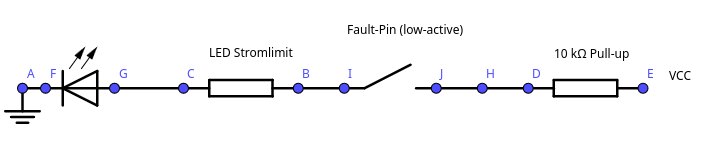
\includegraphics[width=\textwidth]{images/motor_driver_fault_pin.png}
    \caption{Testaufbau des Fault-Pins des Pololu-Motor-Treibers}
    \label{fig:motor_driver_fault_pin}
\end{figure}

Der Fault-Pin ist laut Datenblatt ein Open-Drain-Ausgang, der bei einem Fehler auf Low gezogen wird. Im Testaufbau wurde ein Pull-Up-Widerstand von 10 k$\Omega$ verwendet, um den Pin im Normalfall auf High zu halten. Folgendes Verhalten wurde erwartet: Bei einem Fehler wird der Pin auf Low gezogen und die LED leuchtet auf. Dies war jedoch nicht der Fall. Stattdessen leuchtete die LED dauerhaft, obwohl der Motor einwandfrei funktionierte. Nach Rücksprache mit dem Betreuer stellte sich heraus, dass dieser Pin in der Vergangenheit nie benutzt wurde. Um den Projektfortschritt nicht unnötig zu gefährden, wurde beschlossen, den Fault-Pin nicht weiter zu verwenden und mit der Implementierung des Differential Drive fortzufahren.

\subsection{Low-Level Treiber Test}

Das Testing unterteilte sich in mehrere Schritte. Für die Erstellung der Testfälle wurde dabei zum Großteil KI-generierter Code verwendet. Dadurch konnte der damit verbundene Zeitaufwand signifikant minimiert und zugleich eine ausreichende Testabdeckung garantiert werden. \newline

Zunächst sollte die grundlegende Funktionalität des LL-Treibers getestet werden. Dazu wurden LEDs auf einem Breadboard angebracht, welche die Motoren simulieren sollten. Die Helligkeit der LEDs sollte dabei die Geschwindigkeit des Motors repräsentieren. \newline

Nach erfolgreicher Validierung der Ergebnisse wurde der Testaufbau an die echte Hardware angepasst. Zudem sollte ein Wrapper erstellt werden, der beide Motoren über einzelne Treiber-Objekte anspricht. Dies stellte somit eine Vorstufe zum Differential Drive dar. Ziel war es, die beiden Motoren unabhängig voneinander ansteuern zu können. Dafür wurde das Fahrzeug auf einer Holzkonstruktion bestehend aus zwei Holzlatten platziert. Obwohl die Tests positiv verliefen, sollte sich der Test ohne Bodenkontakt im weiteren Projektverlauf als suboptimal herausstellen.

\subsection{Differential Drive}

- Begriff Differential Drive, woher abgeleitet, was bedeutet es: in unserem Fall beide Reifen je Seite über einen Motor angetrieben, der über Keilrippenriemen an die beiden Reifen angeschlossen ist.

Der Anspruch an die Differential Drive Logik war, eine Logik zur Verfügung zu stellen, um Controllerwerte auf entsprechende Geschwindigkeiten und Richtungen umzurechnen. Nach erfolgreicher Berechnung werden die Werte an eine Queue gesendet werden, die ein Task zyklisch abgreift und letztendlich auf die Motoren appliziert.

\begin{figure}[h]
    \centering
    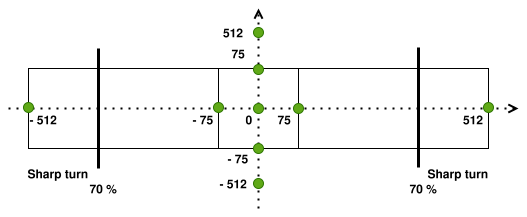
\includegraphics[width=\textwidth]{images/diff_drive_logic.png}
    \caption{Differnetial Drive Logik}
    \label{fig:diff_drive_logic}
\end{figure}

Im Zentrum der Abbildung~\ref{fig:diff_drive_logic} befindet sich die Nullposition. In der Vehicle-Control wird sichergestellt, dass die 

\subsection{Tests}

Wie beim Testing des Low-Level Treibers, wurde der Code auch hier größtenteils KI-generiert. In der Summe gab es zwei Testszenarien:

\begin{itemize}
    \item Logik-Test auf Holzkonstruktion
    \item Logik-Test auf Laborboden
\end{itemize}

Im ersten Fall fielen gleich zu Beginn kleinere Fehler, wie beispielsweise das fehlerhafte Freigeben von Ressourcen, auf. Diese konnten umgehend behoben werden. Trotz der Anpassungen war ein größeres Problem ersichtlich: Die rechte Antriebsseite funktionierte nicht. Der linke Antriebsstrang lief zwar mit der korrekten Geschwindigkeit, dafür passten die Richtungswechsel nicht. \newline

Für Debuggung-Zwecke bietet das verwendete Framework ESP-IDF einen Loggingmechanismus an, der es ermöglicht, den Status von Variablen in Form von Konsolenausgaben nachzuvollziehen. Dafür ist es notwendig, dass der ESP32 über die USB-Schnittstelle mit dem Rechner verbunden ist. \newline

Folgendes Verhalten wurde festgestellt: Die Werte wurden korrekt berechnet, die Queue jedoch nicht richtig abgearbeitet. Das Problem lag bei der Initialisierung der Queue, welche Steuerbefehle entgegennimmt. Die API erlaubt es, Pointer auf Structs oder die komplette Größe des Structs als Queuewerte festzulegen. Im Code wurde beim Laden der Werte aus der Queue das komplette Struct angegeben, beim Laden in die Queue hingegen nur ein Pointer. Aufgrund der Pointergröße konnten nur die ersten 8-Byte richtige Werte enthalten, der Rest enthielt Zufallswerte. Durch Padding/Aligning des Compilers wurde die erste Variable (Speed links, float, 4 Byte) offensichtlich auf 8 Byte skaliert. Dadurch kam es zu dem undefinierten Verhalten, dass nur die linke Seite eine Drehzahl hatte. Die Richtung wurde aus einem Standardwert übernommen. Bei der rechten Seite traf man die Annahme, dass ein Zufallswert aus dem Speicher genommen wurde. Mit großer Wahrscheinlichkeit war dieser außerhalb des Bereichs, weshalb 0 (keine Drehzahl) angenommen wurde. Nach Anpassung des Übergabeparameters liefen beide Motoren mit der gewünschten Geschwindigkeit und die Richtungen entsprechend korrekt gewechselt. \newline

Im zweiten Fall wurde das Fahrzeug auf den Boden des Labors gestellt. Nach einem Timeout von 10 Sekunden sollte das Fahrzeug eine spezifizierte Routine durchlaufen, bei der das Drehverhalten im Stand, Beschleunigen bzw. Abbremsen und gegensätzliches Lenken getestet wurde. Die Beschleunigungstests verliefen durchwegs positiv. Tests, welche hingegen mit einer Drehung des Fahrzeugs bzw. Lenkung in Verbindung standen, wurden nicht erfolgreich abgeschlossen. Erste Versuche, die Ursache zu finden, ließen darauf schließen, dass die Motoren nicht ausreichend Leistung haben, um das Fahrzeug zu drehen. Nach eingehenden Untersuchungen - auch in Verbindung mit dem Betreuer - im Labor wurde festgestellt, dass die zuvor aufgelöteten Widerstände, die den Strom bei 6V Betriebsspannung begrenzen sollten, zu hoch dimensioniert waren. Selbst beim Anlegen einer höheren Spannung von 12V war es nicht möglich, das Fahrzeug zu drehen. Nach Entfernen der Widerstände und Anlegen von 12V Betriebsspannung konnte das Fahrzeug wie gewünscht drehen. \newline

\subsection{Integration}

In diesem Schritt sollte die Ansteuerung der Differential Drive Logik in die Vehicle-Control integriert werden. Die Vehicle-Control ist eine Abstraktionsebene, die als zentrale Anlaufstelle für Befehle vom Controller dient. Darin ist der Haupttask implementiert, der die Steuerbefehle entgegennimmt und an die entsprechenden Queues weiterleitet. Diese Queues werden dann von den Tasks der jeweiligen Komponenten abgearbeitet. Neben der Geschütz- und der Feuersteuerung ist die Ansteuerung der Differential Drive Logik eine der zentralen Komponenten. \newline

Die Integration in die bestehende Vehicle-Control war relativ unkompliziert, da das Abgreifen der Steuerbefehle über den PS4-Treiber einfach handzuhaben ist. Ein Struct enthält alle notwendigen Stick- bzw. Button-Werte, die am Controller gedrückt werden. Problematisch war jedoch der Stick-Drift des linken Sticks, denn dadurch wurde der PS4-Treiber ständig mit Werten versorgt, was zu einer permanenten Anpassung der Geschwindigkeit führte. Die ersten Befehle konnten teilweise noch übermittelt werden, jedoch lief nach kurzer Zeit die Queue über und es kam zu einem Absturz des Programms. \newline

Die Lösung des Problems bestand darin, den Stick-Drift einzudämmen. Daraufhin wurde durch Ausprobieren am Fahrzeug ein Wert ermittelt, ab dem ein neuer Befehl interpretiert werden sollte. Dieser Wert wurde in der Vehicle-Control als Deadzone definiert. Wenn der linke Stick des Controllers innerhalb dieser Deadzone bewegt wird, wird die Geschwindigkeit des Fahrzeugs nicht angepasst. Dadurch wird verhindert, dass die Queue überläuft und das Programm abstürzt. \newline

Allerdings wurde infolgedessen festgestellt, dass die Queue im Stand überläuft, wenn der linke Stick nicht bewegt wird. Das Problem war, dass die Vehicle-Control die Nullposition als normalen Fahrbefehl interpretierte und somit ständig Werte sendete. \newline

Deshalb wurde, wie im Zentrum der Abbildung~\ref{fig:diff_drive_logic} zu sehen, eine Nullposition definiert. Diese wird beim Auftreten, sprich Nicht-Bewegen des linken Sticks, detektiert. Daraufhin wird ein Stop eingeleitet. Sobald dieser abgearbeitet wurde wird ein Flag gesetzt, das anzeigt, dass die Nullposition bereits abgearbeitet wurde. Somit wird verhindert, dass das Stoppen unnötig wiederholt wird und die Queue überläuft. Sobald der linke Stick wieder bewegt wird, wird das Flag zurückgesetzt und die Geschwindigkeit des Fahrzeugs angepasst. \newline

\section{MQTT-Anbindung (Specht)}

Für den Semi-automatischen Modus ist es von zentraler Bedeutung, dass das Fahrzeug Befehle für die Geschützsteuerung empfangen kann. In Abstimmung mit dem Kollegen Jürgens wurde beschlossen, die Kommunikation zwischen KI-Komponente und Fahrzeug über MQTT umzusetzen. MQTT ist ein leichtgewichtiges Publish-Subscribe-Protokoll, das auch in Industrielösungen zum Einsatz kommt. Im ISO/OSI Referenzmodell entspricht es der Anwendungsschicht. In diesem Fall übernimmt der ESP32 die Rolle des Brokers, der über einen zuvor festgelegten Topic Nachrichten empfängt. Die Vehicle-Control wurde so erweitert, dass sie auf den Topic lauscht. Demnach sendet die KI-Komponente Nachrichten an den Broker, die dann von der Vehicle-Control empfangen und verarbeitet werden.

\subsection{WiFi-Stack}

\subsection{MQTT-Stack}

